% ******** Приклад оформлення документа за ДСТУ 3008-95 ********
% ******************** автор: Тавров Д. Ю. *********************

% зазначаємо стильовий файл, який будемо використовувати
\documentclass{udstu}

% починаємо верстку документа
\begin{document}

% створимо титульний аркуш
% за допомогою спеціальної команди
% \maketitlepage{params},
% де params --- це розділені комами пари "параметр={значення}"
\maketitlepage{
% StudentName --- прізвище, ініціали студента
	StudentName={Скорденко Д. О.},
% StudentMale --- стать студента (true, якщо чоловік, false --- якщо жінка)
	StudentMale=true,
% StudentGroup --- група студента
	StudentGroup={КМ-01},
% Title --- назва
	Title={Звіт\\із лабораторної роботи №2\\із дисципліни \invcommas{Розподілені і хмарні обчислення}},
% SupervisorDegree --- науковий ступінь, учене звання керівника роботи
% якщо наукового ступеня немає, можна відповідний рядочок пропустити
	SupervisorDegree={доцент кафедри ПМА},
% SupervisorName --- прізвище, ініціали керівника роботи
	SupervisorName={Ліскін В. О.}
}

% створюємо зміст
\tableofcontents

% створюємо вступ
\intro

\paragraph{\textbf{Мета:}} порівняти однопоточну та багатопоточну версії матричного множення та додавання елементів матриці.

% створюємо перший розділ роботи
\chapter{Основна частина}
\label{chap:1}

\paragraph{\textbf{Опис програми:}}

Для реалізації паралелізму буде використовуватись 'Rayon'.
Для порівняння швидоксті обчислень буде використовуватись 'Criterion'.


\chapter{Опис програми [Тестовий приклад]}
\label{chap:3}

\begin{figure}[!htp]
	\centering
	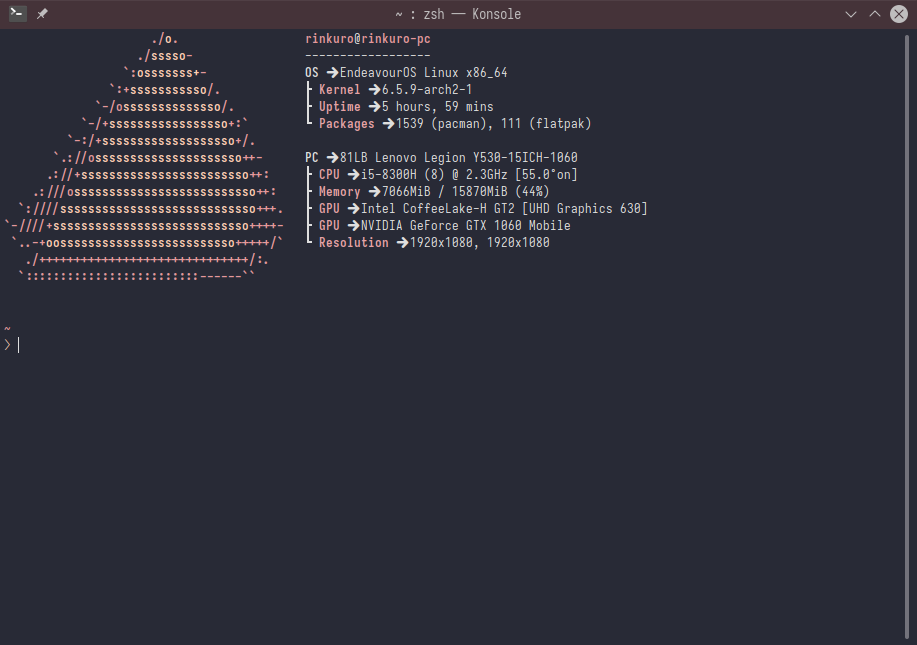
\includegraphics[scale=0.5]{PNG/system-specs.png}
	\caption{Характеристики системи}
	\label{fig:figure1}
\end{figure}

\begin{figure}[!htp]
	\centering
	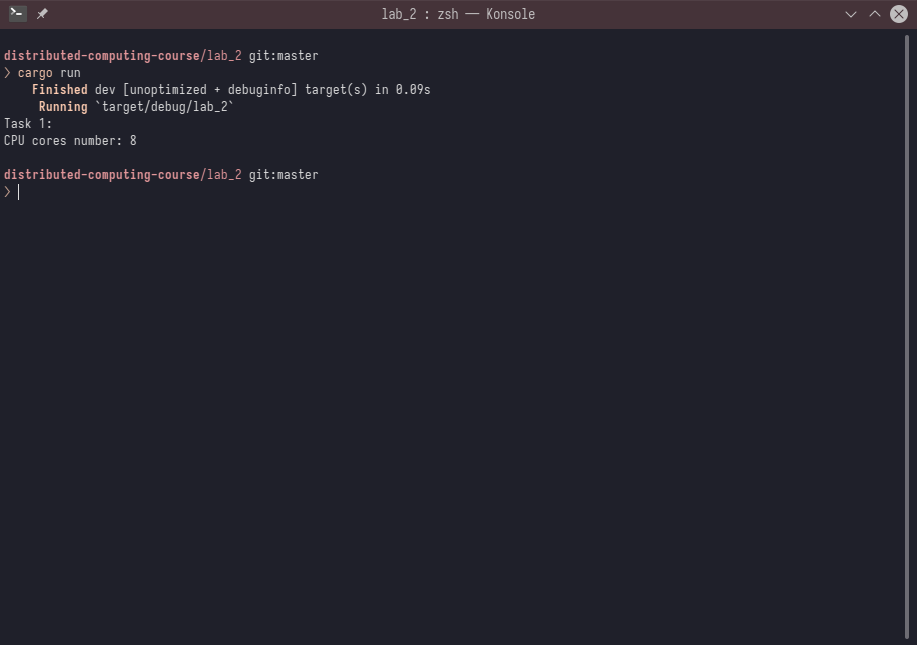
\includegraphics[scale=0.5]{PNG/thread-num-test.png}
	\caption{К-сть ядер процесора}
	\label{fig:figure1}
\end{figure}

\begin{center}
\captionof{table}{Порівняння швидкодії}
\resizebox{\textwidth}{!}{
\begin{tabular}{ | l | c | }
  \hline
  Матричне множення 150x150 (Single thread) & [12.063 ms 12.267 ms 12.480 ms] \\
  Матирчне множення 150x150 (Multi thread) & [3.3324 ms 3.3971 ms 3.4711 ms] \\
  Додавання елементів матриці 1000x1000 (Single thread) & [3.6564 ms 3.6751 ms 3.6963 ms] \\
  Додавання елементів матриці 1000x1000 (Multi thread) & [965.96 µs 990.37 µs 1.0199 ms] \\
  \hline
\end{tabular}
}
\end{center}

% створюємо Висновки
\conclusions

Алгоритми із паралельним обчисленням (Multi thread) в середьому швидші на $50\% - 75\%$.

\append{Код лістінги}

\paragraph{\textsc{*Примітка:}}
У код лістингах при копіюванні втрачається форматування (не копіюються пробіли).
Файли прикріплено до цього pdf (вкладка "прикріплені файли").

\captionof{listing}{matop.rs}
\embedfile[filespec=matop.rs]{../src/matop.rs}
\inputminted{rust}{../src/matop.rs}

\captionof{listing}{lib.rs}
\embedfile[filespec=lib.rs]{../src/lib.rs}
\inputminted{rust}{../src/lib.rs}

\captionof{listing}{main.rs}
\embedfile[filespec=main.rs]{../src/main.rs}
\inputminted{rust}{../src/main.rs}

\end{document}
